\documentclass[tikz, border=4pt]{standalone}

\usepackage{amsmath,amssymb}
\usetikzlibrary{arrows.meta}
\usepackage{xcolor}

\definecolor{utnblue}{RGB}{0, 51, 102}
\definecolor{utnred}{RGB}{204, 0, 0}

\begin{document}
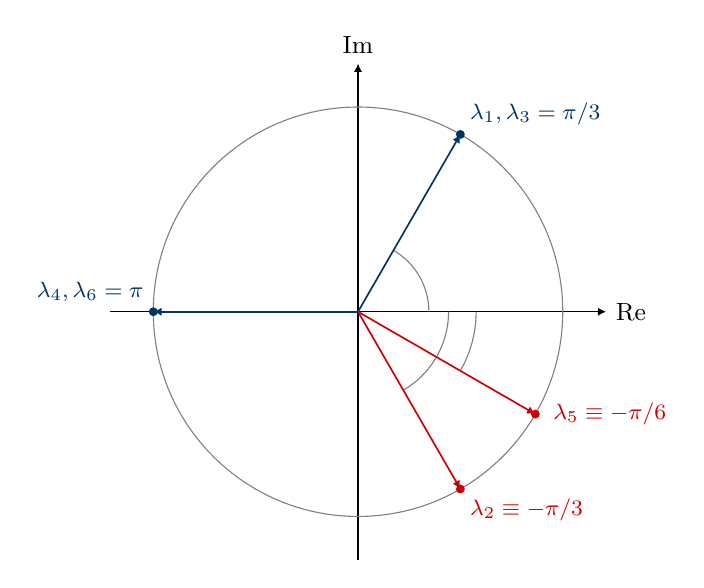
\begin{tikzpicture}[>={Latex[length=3pt,width=3pt]}, font=\small, scale=1.0]

    \def\R{2.6}

    % --- ejes ---
    \draw[->, thin, black] (-\R-0.55,0) -- (\R+0.55,0) node[right] {$\operatorname{Re}$};
    \draw[->, thin, black] (0,-\R-0.55) -- (0,\R+0.55) node[above] {$\operatorname{Im}$};

    % --- circulo unidad ---
    \draw[thin, gray] (0,0) circle (\R);

    % --- arcos de angulo ---
    \draw[gray, thin] (0.9,0) arc (0:60:0.9);
    \draw[gray, thin] (1.15,0) arc (0:-60:1.15);
    \draw[gray, thin] (1.5,0) arc (0:-30:1.5);

    % --- vectores ---
    \draw[->, utnblue, semithick] (0,0) -- (60:\R);
    \draw[->, utnred,  semithick] (0,0) -- (-60:\R);
    \draw[->, utnblue, semithick] (0,0) -- (180:\R);
    \draw[->, utnred,  semithick] (0,0) -- (-30:\R);

    % --- puntos ---
    \fill[utnblue] (60:\R) circle (1.6pt);
    \fill[utnred]  (-60:\R) circle (1.6pt);
    \fill[utnblue] (180:\R) circle (1.6pt);
    \fill[utnred]  (-30:\R) circle (1.6pt);

    % --- etiquetas ---
    \node[utnblue, anchor=south west, font=\footnotesize] at (60:\R)
        {$\lambda_1,\lambda_3=\pi/3$};
    \node[utnred, anchor=north west, font=\footnotesize] at (-60:\R)
        {$\lambda_2\equiv-\pi/3$};
    \node[utnblue, anchor=south east, font=\footnotesize] at (180:\R)
        {$\lambda_4,\lambda_6=\pi$};
    \node[utnred, anchor=west, font=\footnotesize, xshift=3pt] at (-30:\R)
        {$\lambda_5\equiv-\pi/6$};

\end{tikzpicture}
\end{document}
